\documentclass{article}
\usepackage{graphicx}

\title{A computational model investigating Shared Sound Category Learning Mechanisms Hypothesis}
%\subtitle{SOGM project plan, Blok 2}
\author{Akke Houben}
\date{17-02-2015}

\begin{document}
\maketitle
\section{Introduction}
Altough the brainstructures processing speech and music appear to operate independently (left hemisphere being laterized for speech, right hemisphere for music (Kolb \& Whishaw, 1947; Marin \& Perry, 1999; Peretz, 2006)), there are many similarities how the brain is activated while interpreting speech and music (Zatorre et al., 1994; Trehub et al., 199). Especially the learning of sound categorization appear to uttilize similar mechanisms (McMullen \& Saffran, 2004; Hickock \& Poeppel, 2004; Patel, Peretz, et al., 1998). In this project a computational model is designed to investigate the Shared Sound Category Learning Mechanisms Hypothesis. 

\section{Desgin}
First the sound input is transformed to an representation mimicking the cochlear and cortical processing of sounds. The spectrotemporal response fields (STRFs, as shown in Figure 1) of the neurons in the primary auditory cortex (A1) proposed by Taishih Chi, Powen Ru and Shihab A. Shamma (2005) are modelled. These STRF representations are then fed into a machine learning (neural network) algorithm (to be investigated).
The cochlear \& cortical processing and machine learning algorithms will be programmed using C++. A lot of data will have to be processed in a small amount of time and a lot op 'parallel' calculations will be made. A robust and fast program will have to be coded. The programming syntax and methods available with C++ seem to fit my way of thinking and developing. Thus C++ is an easy choice for me.

The test-trial-scheduler will be programmed in an yet to be specified programming language, possibly pyhton, lisp, etc. Here the needed calculations are few and speed is not the main concern. An (relatively) small, easy and transparently programmed programm will suffice.
\begin{figure}
	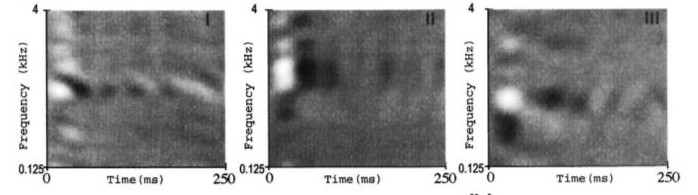
\includegraphics[width=\linewidth]{strfs.jpg}
	\caption{example STRFs from A1 of ferrets (taken from Chi, Ru \& Shamma, 2005)}
	\label{fig:strf}
\end{figure}

\begin{figure}
	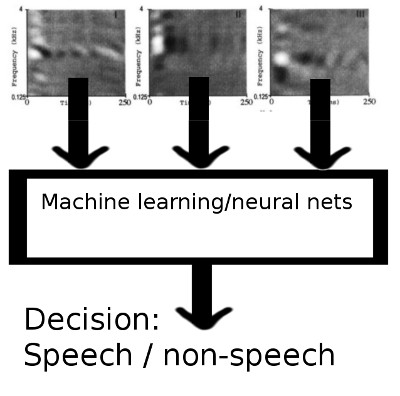
\includegraphics[width=\linewidth]{diagram1.jpg}
	\caption{Processing and machine learning design}
	\label{fig:dia1}
\end{figure}

\begin{figure}
	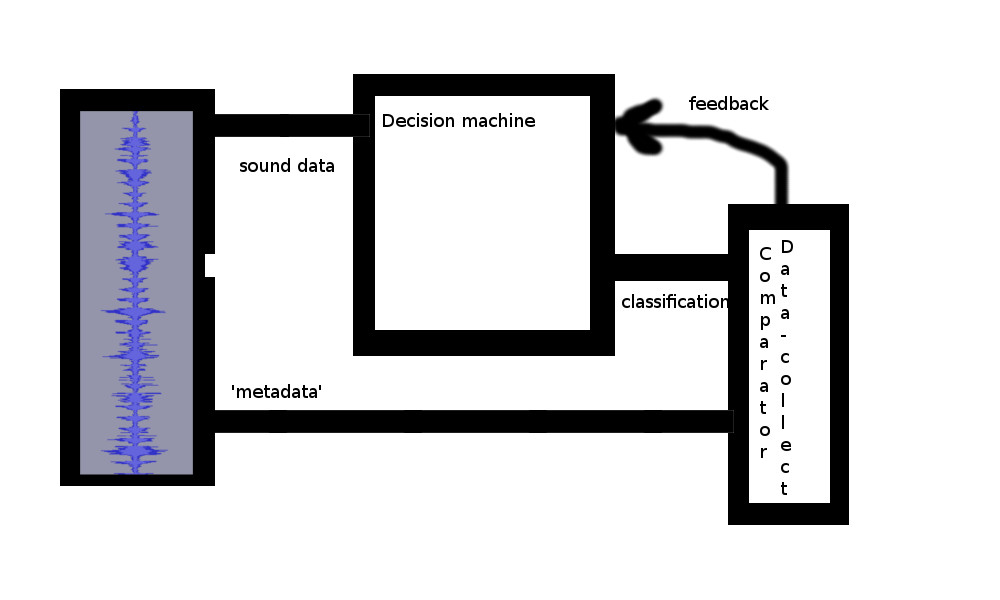
\includegraphics[width=\linewidth]{diagram2.jpg}
	\caption{Scheduler design}
	\label{fig:dia2}
\end{figure}

\section{To do}
\begin{itemize}
	\item program STRFs
	\item Investigate machine learning/neural network possibilities
	\item find a corpus of test data
	\item write trial scheduler
	\item schedule trials and collect data
\end{itemize}
\section{Time schedule}
\begin{itemize}
	\item 24-02 
	\begin{itemize}
		\item cochlear and cortical processing stage programming
		\item investigating what machine learning design will be used
	\end{itemize}
	\item 03-03 
	\begin{itemize}
		\item cochlear and cortical processing programming
		\item decision  what machine learning design will be used
	\end{itemize}
	\item 10-03
	\begin{itemize}
		\item cochlear and cortical processing done
		\item machine learning programming
		\item designing test-trial-scheduler
		\item doing test trials
	\end{itemize}
	\item 17-03
	\begin{itemize}
		\item machine learning algorithm done
		\item trail-scheduler done
		\item trials done, data aquired
	\end{itemize}
\end{itemize}

\section{Goal}
A computational model to investigate the plausibility of  the Shared Sound Category Learning Mechanisms Hypothesis. The program wil consist of 3 major parts: 
\begin{enumerate}
	\item a input processing stage mimicking cochlear and cortical processing mechanisms; 
	\item a machine learning/neural network to learn sound categorization and; 
	\item a test-trial-scheduler which will feed sounds to the system, acquires the responses and displays them in a sensible way.
\end{enumerate}
\end{document}
